% % Created 2015-09-15 Tue 11:46
% \documentclass[11pt]{article}
% \usepackage[utf8]{inputenc}
% \usepackage[T1]{fontenc}
% \usepackage{fixltx2e}
% \usepackage{graphicx}
% \usepackage{longtable}
% \usepackage{float}
% \usepackage{wrapfig}
% \usepackage{rotating}
% \usepackage[normalem]{ulem}
% \usepackage{amsmath}
% \usepackage{textcomp}
% \usepackage{marvosym}
% \usepackage{wasysym}
% \usepackage{amssymb}
% \usepackage{hyperref}
% \usepackage{color}
% \usepackage{soul}
% \tolerance=1000
% \usepackage[margin=1in]{geometry}

% \newcommand{\hilight}[1]{\colorbox{yellow}{#1}}

% %\author{Alex Ansari}
% %\date{}
% %\title{TALOS}
% %\hypersetup{
% %  pdfkeywords={},
% %  pdfsubject={},
% %  pdfcreator={Emacs 24.3.1 (Org mode 8.2.10)}}


% \begin{document}
\section{RoboKnee}

The RoboKnee device was built as a prototype system to enhance human strength, endurance and speed.  The main design objectoves in the RoboKnee system were to enhance human performance using a low-impedance mechanical system that incorporates a natural user interface, long life, and is comfortable to wear.  The main control objective of the suit is to provide a ``get out of the way" control scheme, wear the system inherently interacts with the user through a low-impedance interface.  

The design of a linear series elastic actuator and a novel control method for controlling a single powered joint at the knee of the operator are presented in this section.

\subsection{Actuator specifications}

The RoboKnee actuator was designed to specifically provide low impedance and high force feedback fidelity.  Series elastic actuators are a more robust option for measuring output forces and torques than using notoriously delicate and expensive load cells.  


The actuator used in the RoboKnee device is shown in Figure \ref{fig:roboAct}.  The actuator consists of a drive train subassembly and an output carriage subassembly. The two subassemblies are coupled through die compression springs.  A servo motor directly drives a ball screw assembly to drive a ball nut flange which pushes on a spring retaining plate.  Secondary spring retaining plate is coupled to an output assembly.  Measuring the deflection in the die springs makes it possible to measure the force applied to the output of the linear SEA.  
\begin{figure}[thpb]
\centering
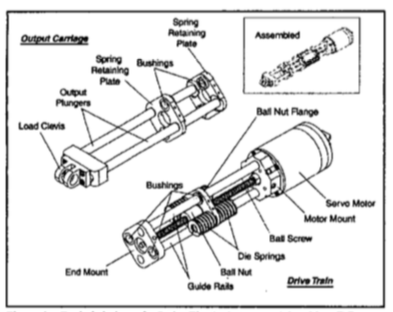
\includegraphics[width=3.in]{exos/figs/roboKnee/roboSEA}
  \caption{}
  \vspace{-0.2in}
 \label{fig:roboAct}   
 \end{figure}

The linear actuator pictured in Figure \ref{fig:roboAct} { \bf weighs 1.13 kg, has a stroke length of 30.5 cm and diameter of 5.8 cm}.  The {\bf maximum speed of the actuator is 28 cm/s}.  The actuators {\bf maximum continuous force is 565N, with a peak maximum force of 1330 N}, with {\bf maximum continuous power of 164 W, and maximum peak power of 634 W}.   

The force control bandwidth of the RoboKnee actuator is dependent on the magnitude of the force, as significant time delays can occur for larger forces due to the fact that there is an inherent time delay due to the time it takes for the spring to compress.  Thus, the {\bf small force control bandwidth of the system is 35 Hz} and the {\bf high force bandwidth is around 7.5 Hz}. 
 
 \subsection{Exoskeleton Specifications}
 
 The RoboKnee mechanism consists of a single actuated degree of freedom at the flexion/extension joint of the operator.  Note that the mechanism itslef does not provide a pathway for transferring weight from a load directly to the ground.  The mechanism transfers loads directly to the users musculoskeletal structure, and focuses primarily on augmenting the torque supplied to the users knee joint.
 
 The RoboKnee mechanism itself is composed of an off-the-shelf knee brace modified with structural pieces to extend the brace and provide actuator attachment points.  The RoboKnee mechanism is shown in \ref{fig:roboKnee}.  
 \begin{figure}[thpb]
\centering
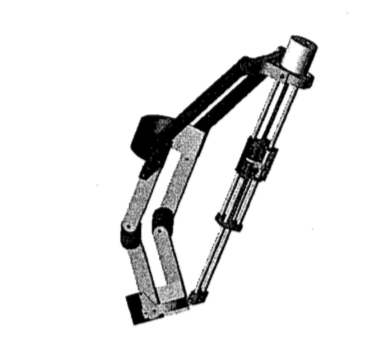
\includegraphics[width=3.in]{exos/figs/roboKnee/roboBrace}
  \caption{}
  \vspace{-0.2in}
 \label{fig:roboKnee}   
 \end{figure}
 There exact length between attachment points of the actuator is not listed in the literature, but it appears that the attachment points are at minimum the stroke displacement of the actuator  away from each other, so a {\bf minimum moment arm of 30.5 cm} is a reasonable approximation.
 
 The RoboKnee mechanism uses a linear potentiometer spanning the spring retaining plates to measure displacement in the springs and subsequently to measure force at the actuator output.  The forces between the users foot and the ground are also measured using single axis load cells.  Potentiometers which measure the knee joint angle are also employed in this design.     
 
 The single actuator as well as control and sensor electronics are run using {\bf 4 kg of nickel-metal-hydride batteries, which give the system only about 30-60 minutes of heavy use}.
 
 
 \subsection{Control Specifications}
 
 The control scheme for the RoboKnee device is a hierarchical approach, which uses a straightforward mid-level force generation scheme coupled with a low-level closed-loop force-based control loop.  The low-level, or rather joint level control is a PD control loop.
 
 The mid-level controller of the RoboKnee uses several simplifying assumptions to perform ``force amplification" to offload a percentage of the torque required by the user to actuate the system's knee joint.  This is achieved through a positive force feedback amplification which is based on measuring the ground reaction force and using this value to calculate the torque that would be required to produce this force in a static situation, namely, \[ \tau = R \times F,\] where $R$ is the vector from the ground reaction force to the users knee and $F$ is the ground reaction force.  Note that in the RoboKnee implementation this value can only be estimated due to the fact that the ankle joint angle and the ground reaction force is assumed to be purely vertical (which is a result of the single axis force sensors on the users feet).
   
   
 Once the estimated joint torque $\tau$ is calculated, an amplification factor is used in the RoboKnee control scheme to decide how much of the required knee torque will be provided by the control system.  For example, if the amplification factor were chosen to be one the actuator would completely compensate for the sensed ground reaction forces, and if it were set to zero to exoskeleton would provide no force.
  
 
 \subsection{Opinion} 
 
 The RoboKnee is a relatively simple system that highlights several intelligent hardware and control design concepts.  The use of a linear ball screw with a series elastic element that enables high-fidelity force control is a very good idea. The idea of using the measured ground reaction forces to produce the desired knee joint torque is also interesting in the sense that it is very simple and relies on a minimal amount of information.
 
 The overall design of the RoboKnee mechanism is most likely not the greatest, as it significantly increases the effective volume of the operator-system leg, but as a prototype this concept offers interesting benefits.
 
 % \end{document}
 
 % Jerry E. Pratt and Benjamin T. Krupp and Christopher J. Morse and Steven Collins, "The RoboKnee: An Exosskeleton for Enhancing Strength and Endurance During Walking," International Conference on Robotics and Automation, 2004, pp. 2430-2435.
 
 
 